\documentclass[conference]{IEEEtran}
\IEEEoverridecommandlockouts
\usepackage[utf8]{inputenc}                   
\usepackage[spanish]{babel}  
\usepackage{cite}
\usepackage{amsmath,amssymb,amsfonts}
\usepackage{algorithmic}
\usepackage{graphicx}
\usepackage{textcomp}
\usepackage{xcolor}
\usepackage{listings}
\usepackage{geometry}                         
\geometry{left=18mm,right=18mm,top=21mm,bottom=21mm}
\usepackage{ucs}
\usepackage{amsmath}
\usepackage{amsfonts}
\usepackage{amssymb}
\usepackage{graphicx}
\usepackage[lofdepth,lotdepth]{subfig}
\usepackage{unitsdef}
\usepackage{pdfpages} 
\renewcommand{\unitvaluesep}{\hspace*{4pt}}	
\usepackage[colorlinks=true,urlcolor=purple,linkcolor=black,citecolor=black]{hyperref} 
\usepackage{float}	
\usepackage{booktabs}
\batchmode
\bibliographystyle{plain} 
\pagestyle{plain} 
\pagenumbering{arabic}
\usepackage{lastpage}
\usepackage{fancyhdr}	
\pagestyle{fancy}	
\usepackage{multicol} 


\def\BibTeX{{\rm B\kern-.05em{\sc i\kern-.025em b}\kern-.08em
T\kern-.1667em\lower.7ex\hbox{E}\kern-.125emX}}

\cfoot{\textbf{\thepage}}


\begin{document}

%plantilla imprimir codigo Java
\lstnewenvironment{javaCode}[1][]
{\lstset{
    language=Java,
    basicstyle=\footnotesize\ttfamily,
    numbers=left,
    numberstyle=\tiny,
    stepnumber=1,
    numbersep=5pt,
    keywordstyle=\color{blue},
    commentstyle=\color{gray},
    stringstyle=\color{purple},
    breaklines=true,
    breakatwhitespace=true,
    tabsize=4,
    showspaces=false,
    showstringspaces=false,
    frame=single,
    captionpos=b,
    #1
}}
{}

\title{
\includegraphics[width=8cm]{imagen/itsoeh.png}\\ \vspace*{0.2cm} {\large Instituto Tecnológico Superior del Occidente del Estado de Hidalgo} \\
  \vspace*{0.2cm}
  \large Ingeniería en Tecnologías de la Información y Comunicaciones  \\  
  \vspace*{0.5cm}  
  {\huge Proyecto Integrador} \\
  {\normalsize Prototipo de problemas de solución de ingeniería aplicado a primer semestre}\\
  {\vspace{1cm} \large \textbf{Coordinador del proyecto:}\\ Dr. Francisco Javier Cuadros Romero}\\
  \vspace{1cm}
  {\large \textbf{Integrantes del equipo:}}
  \vspace{0.5cm}
  }
  
\author
{\IEEEauthorblockN{1\textsuperscript{er} Cruz Granados Dulce Marina}%primer autor
\IEEEauthorblockA{\textit{Estudiante de ITIC´s} \\
\textit{ITSOEH}\\
Tezontepec de Aldama, Hgo. \\
230110477@itsoeh.edu.mx}
\and
%segundo autor
\IEEEauthorblockN{2\textsuperscript{do} Fuentes Pérez Bryan}
\IEEEauthorblockA{\textit{Estudiante de ITIC´s} \\
\textit{ITSOEH}\\
El Rosario, Hgo. \\
230110581@itsoeh.edu.mx}
\and
%segundo autor
\IEEEauthorblockN{3\textsuperscript{er}Hernández Monroy Ricardo}
\IEEEauthorblockA{\textit{Estudiante de ITIC´s} \\
\textit{ITSOEH}\\
Tezontepec de Aldama, Hgo. \\
230110240@itsoeh.edu.mx}
\and
%segundo autor
\IEEEauthorblockN{4\textsuperscript{to} Salazar Guerrero Diego}
\IEEEauthorblockA{\textit{Estudiante de ITIC´s} \\
\textit{ITSOEH}\\
San Salvador, HGO. \\
230110580@itsoeh.edu.mx}
\and
%segundo autor
\IEEEauthorblockN{5\textsuperscript{to} Santiago Reséndiz Melanie}
\IEEEauthorblockA{\textit{Estudiante de ITIC´s} \\
\textit{ITSOEH}\\
Actopan, HGO. \\
230110616@itsoeh.edu.mx}
 }
 \maketitle

 \onecolumn
 \tableofcontents
 \newpage
 \twocolumn





\begin{abstract}
During the period from August to December 2023, we covered different subjects in the Information and Communication Technology Engineering program. In each of these subjects, the exercises to be solved were complemented and related. In differential calculus, the first three exercises were addressed: equation of a line, quadratic equation, and point on a circumference. In the discrete mathematics subject, the following three problems were discussed: conversion of negative or positive decimal integers to binary, conversion of binary numbers to decimal, and truth tables. In the ethics subject, a connection was established with references and research fundamentals, delving deeper into the study of these exercises. In the Introduction to ICT subject, knowledge was applied to topics such as the use of repositories. Finally, in the programming subject, the solutions to the problems were coded.
\end{abstract}

\begin{IEEEkeywords}
recta, interseccion, coordenada, punto
\end{IEEEkeywords}

\section{Introducción}
En el siguiente documento se hablará sobre seis problemas aplicados al primer semestre de Ingenieria en Tecnologías de la Información y Comunicaciones creando programas en JAVA.

El primer problema habla sobre la pediente de la recta en el cual dadas las coordenadas  $(x1,y1)$ y $(x2,y2)$ al igual que los puntos A y B nos regrese la ecuación de la recta y el ángulo interno que se forma entre el eje horizontal y la recta. El segundo problema es encontrar las raíces de una ecuación de grado dos o ecuación cuadrática de la forma $ax^2+bx+c=0$. El tercer problema nos pide sdeterminar si un punto en el plano cartesiano está dentro o fuera de una circunferencia con centro fuera del origen y de un radio r. El  cuarto problema requiere comprender la numeración binaria para así poder crear el programa que nos haga la conversión de un número decimal a un número binario equivalente. El quinto  problema es parecido al anterior solo que viceversa, ahora es encontrar el número decimal equivalente a un número binario dado por el usuario. El sexto problema nos pide que dados ciertos números de bits se cree una tabla de verdad correspondiente a la cantidad de bits ingresada por el ususario.\\

Estos seis problemas matemáticos que se presentan a continuación en este informe fueron resueltos con la metodología de las 6Ds que consiste en dar primero una \textbf{D}efinición del problema o información acerca del tema que aborda el problema, después \textbf{D}escribir el problema que queremos solucionar, luego de ello \textbf{D}iseñar una solución analizando los datos dados, para después \textbf{D}esarrollar la solución paso por paso y mencionando el código hecho en JAVA para cada problema, y continuar con \textbf{D}epuración y pruebas que consiste en generar una tabla de corridas o compilaciones del código, para terminar con la útlima D que es \textbf{D}ocumentar todo lo anterior, lo cual se muestra a continuación.

\section{Objetivos}
\subsection{Objetivo General}
\begin{itemize}
    \item El objetivo general del uso de software de resolución de problemas de ingeniería es mejorar la eficiencia y efectividad en la resolución de desafíos técnicos y científicos en el campo de la ingeniería, a través de la utilización de herramientas informáticas especializadas.
\end{itemize}

\subsection{Objetivos específicos}
\begin{enumerate}
    \item Adquirir conocimientos sobre las características y funcionalidades de diferentes software de resolución de problemas de ingeniería utilizados en el campo específico de estudio.
    \item Familiarizarse con la interfaz y la forma de operar de los software seleccionados, incluyendo la entrada de datos, la selección de algoritmos y la interpretación de resultados.
    \item Aplicar el software en el modelado y diseño de sistemas y componentes, con el fin de optimizar su funcionamiento y mejorar su eficiencia.
    \item Utilizar el software para realizar análisis de datos y visualización de resultados, con el fin de tomar decisiones fundamentadas y extraer conclusiones relevantes.
    \item Desarrollar habilidades para la resolución de problemas técnicos mediante la aplicación de software de ingeniería, incluyendo la identificación de variables clave, la formulación de hipótesis y la realización de experimentos virtuales.
    \item Promover el trabajo en equipo y la colaboración utilizando el software, permitiendo compartir proyectos, datos y resultados entre diferentes miembros del equipo.
    \item Desarrollar habilidades de comunicación técnica al presentar y explicar los resultados obtenidos mediante el software de resolución de problemas de ingeniería.
    \item Fomentar la actualización y el aprendizaje continuo sobre nuevas herramientas y técnicas de software de ingeniería, para estar al tanto de los avances tecnológicos en el campo.
    \item Preparar a los estudiantes para enfrentar los desafíos del mundo laboral en ingeniería, donde el uso de software de resolución de problemas es una habilidad altamente demandada.
\end{enumerate}


\section{Ecuación de la recta}
\subsection{Definición}
Dados 2 puntos A y B con coordenadas $(x1, y1)$ y
$(x2, y2)$ respectivamente. Regresar la ecuación de la recta y el ángulo interno $\alpha$ que se forma entre el eje horizontal y la recta.

\subsection{Descripción del problema}

En este problema, se tienen dos puntos $A$ y $B$ con coordenadas $(x_1, y_1)$ y $(x_2, y_2)$ respectivamente. El objetivo es calcular la ecuación de la recta que pasa por estos puntos y determinar el ángulo interno $\alpha$ que dicha recta forma con el eje horizontal.

\subsection{Diseño de la solución}

La ecuación de la recta se obtiene utilizando la fórmula de la pendiente:

\begin{equation}
m = \frac{y_2 - y_1}{x_2 - x_1}
\end{equation}

Una vez obtenida la pendiente $m$, el ángulo interno $\alpha$ se puede calcular utilizando la función trigonométrica arcotangente:

\begin{equation}
\alpha = \arctan(m)
\end{equation}

\subsection{Desarrollo de la solución}

Para resolver el problema, se puede utilizar un programa en JAVA. A continuación se muestra un ejemplo de código:

\begin{javaCode}
import java.util.Scanner;

public class recta {
    public static void main(String[] args) {
        Scanner scanner = new Scanner(System.in);

        System.out.println("Ingrese las coordenadas del punto A:");
        System.out.print("x1: ");
        double x1 = scanner.nextDouble();
        System.out.print("y1: ");
        double y1 = scanner.nextDouble();

        System.out.println("Ingrese las coordenadas del punto B:");
        System.out.print("x2: ");
        double x2 = scanner.nextDouble();
        System.out.print("y2: ");
        double y2 = scanner.nextDouble();

        // Calcular la pendiente de la recta
        double pendiente = (y2 - y1) / (x2 - x1);

        // Calcular el ángulo en radianes
        double anguloRadianes = Math.atan(pendiente);

        // Convertir el ángulo a grados
        double anguloGrados = Math.toDegrees(anguloRadianes);

        // Calcular el ángulo interno α entre el eje horizontal y la recta
        double anguloInterno = 90 - anguloGrados;

        // Calcular el punto de intersección con el eje y (cuando x = 0)
        double puntoInterseccionY = y1 - pendiente * x1;

        // Construir la ecuación de la recta en formato y = mx + b
        String ecuacionRecta = "y = " + pendiente + "x + " + puntoInterseccionY;

        System.out.println("Ecuación de la recta: " + ecuacionRecta);
        System.out.println("Ángulo interno α: " + anguloInterno + "grados");
        System.out.println("Punto de intersección con el eje y: (0, " + puntoInterseccionY + ")");
        System.out.println("Pendiente = "+pendiente);
       
    }
}
\end{javaCode}

\subsection{Depuración y pruebas}

Durante el desarrollo y ejecución del programa, es posible encontrar errores o problemas. Para depurar el programa, se pueden utilizar técnicas como la impresión de mensajes de depuración, el uso de herramientas de depuración y la revisión del código en busca de posibles errores. Luego de depurar el programa, se puede proceder a realizar pruebas para verificar su funcionamiento correcto.

En el cuadro 1 se muestran los resultados obtenidos al compilar el código.\\

\begin{table}[!ht]
\label{T:equipos}
\begin{center}
\begin{tabular}{| c | c | c | c | c | c | c |}
\hline
\textbf{$x_1$} & \textbf{$x_2$} & \textbf{$y_1$} & \textbf{$y_2$} & \textbf{Pendiente} & \textbf{Inclinación} & \textbf{Intersección} \\
\hline
2 & 4 & 4 & 6 & 1 & 45$^o$ & -2 \\
3 & 2 & 4 & 1 & 3 & 71.57$^o$ & -5 \\
2 & 2 & 2 & 2 & 0 & 0$^o$ & 0 \\
1 & 3 & 2 & 4 & 1 & 45$^o$ & 1 \\
\hline
\end{tabular}
\caption{Tabla de corridas.}
\end{center}
\end{table}

\section{Raíces de una Ecuación Cuadrática}

\subsection{Definición}
Es una expresión que puede aplicarse para calcular el valor de una variable a partir de determinados datos.
Usualmente, con fórmula general se hace referencia a aquella que permite resolver ecuaciones cuadráticas, es decir, ecuaciones de segundo grado. Estas son aquellas donde el máximo exponente al que está elevada la incógnita es 2 y que tiene la siguiente forma:
\begin{equation}
    ax^2 + bx + c = 0
\end{equation}\\
Resolverla significa encontrar todos aquellos números reales, que cumplen la igualdad cuando sustituyen a $x$ en la ecuación. Cada uno de esos números, se llama solución de la ecuación. También es frecuente llamarles raíces o ceros de la ecuación.
Tomando como referencia la ecuación 3, la fórmula general para resolver la ecuación es la siguiente:
\begin{equation}
    x_{1, 2} = \frac{-b \pm \sqrt{b^2-4ac}}{2a}
\end{equation}\\
 Se observa que hay dos posibles soluciones, una por cada signo de la raíz cuadrada, por esto la $x$ aparece con dos subíndices: uno por cada solución.
 Le llamamos  discriminante a la expresión que se encuentra dentro de la raíz: $ b^2-4ac $, este discriminante nos permitirá determinar si las soluciones de la ecuación se encuentran dentro del conjunto de los números reales ($\mathbb{R}$) o en el conjunto de los números complejos ($\mathbb{C}$), establecido por el signo de este.\cite{FormulaGeneral} \\
\begin{figure}[h!]
\centering
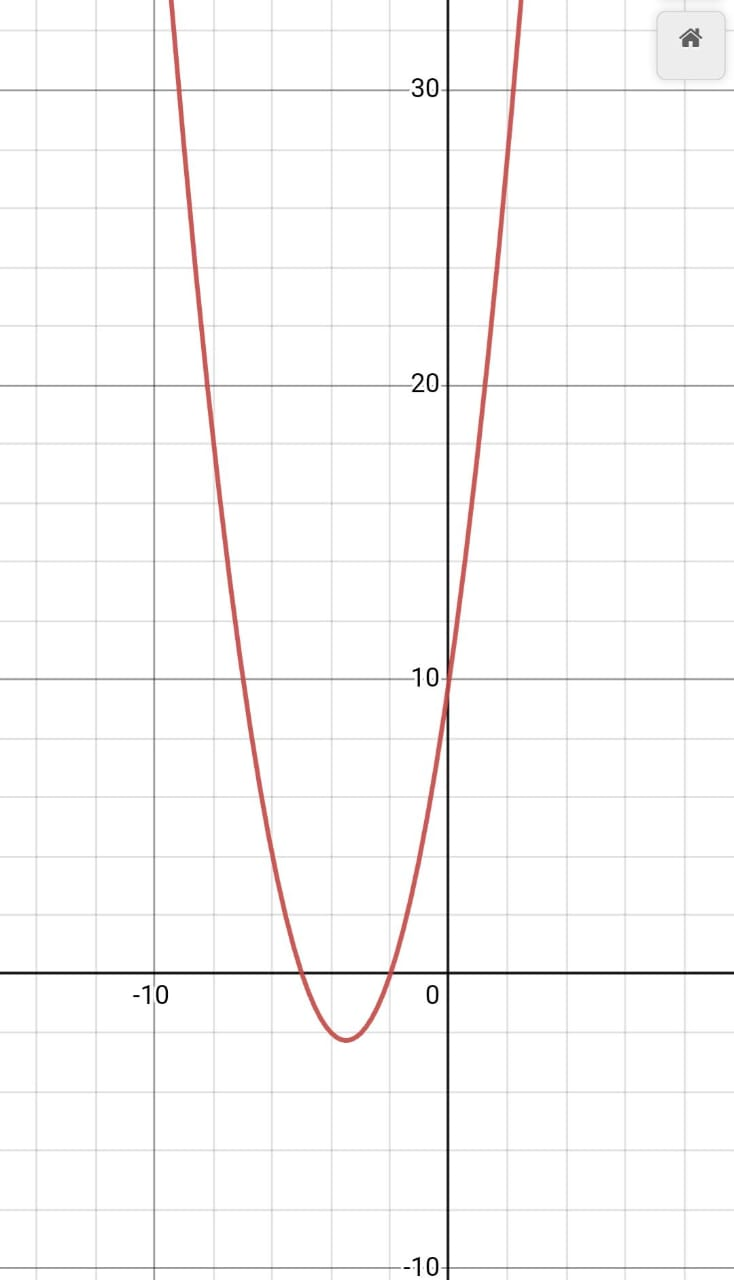
\includegraphics[width=4.5cm]{imagen/hola.jpg}
\caption{Gráfica de una ecuación cuadrática.}
\label{fig:grafica}
\end{figure}
\\

 \subsection{Descripción del problema}
Dada una ecuación cuadrática regresar los valores de las raíces en caso de que estén sobre el conjunto de los números reales, en caso contrario indicar que la solución está en el conjunto de los números complejos.

\subsection{Diseño de solución}
El discriminante que definiremos como $ D = b^2 - 4ac$ determina la naturaleza de las raíces:
\begin{itemize}
    \item Si $D > 0$, las raíces son números reales distintos.
    \item Si $D = 0$, las raíces son números reales iguales.
    \item Si $D < 0$, las raíces son números complejos conjugados.
\end{itemize}

\subsection{Desarrollo de solución}

\begin{javaCode}

        System.out.print("Coeficiente a: ");
        double a = input.nextDouble();
        System.out.print("Coeficiente b: ");
        double b = input.nextDouble();
        System.out.print("Coeficiente c: ");
        double c = input.nextDouble();
        double discriminante = b * b - 4 * a * c;
        if (discriminante > 0) {
            double raiz1 = (-b + Math.sqrt(discriminante)) / (2 * a);
            double raiz2 = (-b - Math.sqrt(discriminante)) / (2 * a);
            System.out.println("Las raices son numeros reales distintos:");
            System.out.println("Raiz 1: " + raiz1);
            System.out.println("Raiz 2: " + raiz2);
        } else if (discriminante == 0) {
            double raiz = -b / (2 * a);
            System.out.println("Las raices son numeros reales iguales:");
            System.out.println("Raiz: " + raiz);
        } else {
            System.out.println("Las raices son numeros complejos conjugados.");
        }

\end{javaCode}

\subsection{Depuración y pruebas}

\begin{table}[!ht]
\label{T:equipos}
\begin{center}
\begin{tabular}{| c | c | c | c | c |}
\hline
\textbf{$a$} & \textbf{$b$} & \textbf{$c$} & \textbf{$x_1$} & \textbf{$x_2$} \\
\hline
1 & 1 & 1 & Complejos & Complejos \\
1 & 10 & 25 & -5 & -5 \\
3 & -5 & 2 & 1 & 2/3\\
6 & -36 & 0 & 6 & 0 \\
1 & 2 & 3 & Complejos & Complejos \\
\hline
\end{tabular}
\caption{Tabla de corridas.}
\end{center}
\end{table}

En el cuadro 1 se muestra una tabla de pruebas con diferentes valores en $a$, $b$ y $c$ en las tres primeras columnas, y el valor de las raíces arrojadas por el programa, en las dos últimas columnas.

\section{Punto en una Circunferencia}

\subsection{Definición}
El objetivo de este problema de la ingeniería es determinar la inclusión de un punto T, definido por sus coordenadas $(x_2, y_2)$, en el área de una circunferencia específica. Esta posee un centro en el punto C, con coordenadas $(x_1, y_1)$, y un radio de longitud $r$. Se evalúa si el punto T se encuentra dentro del perímetro de la circunferencia o si, por el contrario, se ubica fuera de dicho perímetro

\begin{equation}
\text{distancia} = \sqrt{(x_2 - x_1)^2 + (y_2 - y_1)^2}
\end{equation}

Resulta necesario llevar a cabo una comparación exhaustiva entre la distancia que separa al centro de la circunferencia y el punto T, y la longitud del radio. Si la distancia obtenida resulta ser menor o igual a la longitud del radio, se puede concluir que el punto T se encuentra ubicado dentro de los límites de la circunferencia. Por el contrario, si la distancia es mayor a la longitud del radio, se establece que el punto T se encuentra situado en una posición exterior con respecto a la circunferencia.

\subsection{Descripción del problema}

Dada una circunferencia con centro en el punto C con coordenadas $(x_1, y_1)$ y radio $r$, evaluar si un punto T con coordenadas $(x_2, y_2)$ está dentro del área de la circunferencia.

\subsection{Diseño de solución}

La distancia entre el centro $C$ y el punto $T$ se calcula utilizando la fórmula de la distancia entre dos puntos en el plano la cual se define como anteriormente en la ecuación 5.

 \begin{figure}[h!]
\centering
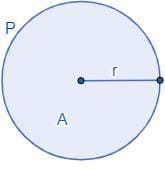
\includegraphics[width=6cm]{imagen/Imagen de WhatsApp 2023-11-23 a las 21.07.09_8c5cc9f6.jpg}
\caption{Gráfica de una circunferencia}
\label{fig:grafica}
\end{figure}

\subsection{Desarrollo de solución}

\lstset{
  language=Java,
  basicstyle=\ttfamily,
  keywordstyle=\bfseries,
  commentstyle=\itshape,
  showstringspaces=false,
  columns=flexible,
  frame=single,
  numbers=left,
  numberstyle=\tiny,
  breaklines=true,
  captionpos=b
}

\begin{javaCode}




        Scanner scanner = new Scanner(System.in);

        System.out.println("Ingrese la coordenada x1");
        double x1 = scanner.nextDouble();
        System.out.println("Ingrese la coordenada y1");
        double y1 = scanner.nextDouble();

        System.out.println("Ingrese el radio de la circunferencia (r):");
        double r = scanner.nextDouble();

        System.out.println("Ingrese la coordenada a evaluar con el punto x2");
        double Tx2 = scanner.nextDouble();
        System.out.println("ingrese la coordenada a evaluar con el punto y2");
        double Ty2 = scanner.nextDouble();

        double distancia = Math.sqrt(Math.pow(Tx2 - x1, 2) + Math.pow(Ty2 - y1, 2));

        if (distancia <= r) {
            System.out.println("El punto se encuentra dentro del area de la circunferencia.");
        } else {
            System.out.println("El punto esta fuera del area de la circunferencia.");
        }
    }
    
}

\end{javaCode}
\\
\subsection{Depuración y pruebas}
En el cuadro 2 se muestran los resultados obtenidos al compilar el código en JAVA de este problema.
\begin{table}[!ht]
\label{T:equipos}
\begin{center}
\begin{tabular}{| c | c | c | c | c | c |}
\hline
\textbf{$x_1$} & \textbf{$y_1$} & \textbf{$r$} & \textbf{$x_2$} & \textbf{$y_2$} & \textbf{Afuera o Adentro}\\
\hline
1 & 2 & 4 & 2 & 1 & Adentro \\
3 & 4 & 2 & 2 & 1 & Afuera \\
1 & 6 & 4 & 4 & 5 & Adentro \\
7 & 4 & 10 & -5 & -3 & Afuera\\
-4 & -5 & 6 & -7 & -8 & Adentro\\
\hline
\end{tabular}
\caption{Tabla de corridas.}
\end{center}
\end{table}



\section{Conversion de decimal a binario con signo}

\subsection{Definicion de la solución}

El problema planteado consiste en obtener el equivalente binario de un número decimal con signo. Se debe respetar la regla de conversión de complemento a dos para los números negativos, con el objetivo de diseñar un algoritmo capaz de tomar cualquier número decimal como entrada y devolver su representación binaria correspondiente.\cite{Decimal a  binario con signo}
\subsection{Descripción del problema}
Dado un numero decimal entero positivo o negativo regresar su equivalente en binario.

\subsection{Diseño de la solucion}
Para diseñar una solución viable al progreso del algoritmo, necesitaremos establcer los siguinetes pasos:

\begin{enumerate}

\item Definir el número decimal para después convertir a binario.

\item Invertir los \texttt{bits}.

\item Sumar 1 al \texttt{bit} menos significativo. Así obtendremos el complemento a dos.
\end{enumerate}

 \begin {figure}[h!]
\centerline{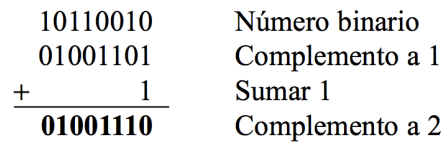
\includegraphics[width = 5cm]{imagen/ejemploa2.png}}
\caption{Procedimineto del complemento a dos.}
\label{fig}
\end {figure}

\subsection{Desarrollo de la solución}
Se presentará el algoritmo, desarrollado en el lenguaje de programación JAVA.

\lstset{
  language=Java,
  basicstyle=\ttfamily,
  keywordstyle=\bfseries,
  commentstyle=\itshape,
  showstringspaces=false,
  columns=flexible,
  frame=single,
  numbers=left,
  numberstyle=\tiny,
  breaklines=true,
  captionpos=b
}

\begin{javaCode}


import java.util.Scanner;
public class Ejercicio4 {

  
    public static void main(String[] args) {
        //entrada
             Scanner entrada = new Scanner(System.in);

        // Solicitar al usuario que ingrese un número decimal
        System.out.print("Ingrese un número decimal: ");
        int numeroDecimal = entrada.nextInt();

        // Verificar si el número es negativo
        boolean esNegativo = false;
        if (numeroDecimal < 0) {
            esNegativo = true;
            numeroDecimal = Math.abs(numeroDecimal);
        }

        // Inicializar una cadena para almacenar el número binario
        String numeroBinario = "";

        // Manejar el caso especial cuando el número decimal es 0
        if (numeroDecimal == 0) {
            numeroBinario = "0";
        } else {
            // Convertir el número decimal a binario
            while (numeroDecimal > 0) {
                int residuo = numeroDecimal % 2; // Obtener el residuo de la división por 2
                numeroBinario = residuo + numeroBinario; // Agregar el residuo al inicio de la cadena binaria
                numeroDecimal = numeroDecimal / 2; // Dividir el número decimal por 2
            }

            // Calcular el complemento a dos si el número es negativo
            if (esNegativo) {
                StringBuilder complementoBuilder = new StringBuilder();
                boolean encontradoPrimerUno = false;

                // Invertir los bits
                for (int i = numeroBinario.length() - 1; i >= 0; i--) {
                    char bit = numeroBinario.charAt(i);
                    if (!encontradoPrimerUno) {
                 
                        if (bit == '1') {
                            encontradoPrimerUno = true;
                        }
                        complementoBuilder.insert(0, bit);
                    } else {
                        // Invertir los bits restantes
                        if (bit == '0') {
                            complementoBuilder.insert(0, '1');
                        } else {
                            complementoBuilder.insert(0, '0');
                        }
                    }
                }

                numeroBinario = complementoBuilder.toString();
            }
        }

        // Agregar signo negativo si corresponde
        if (esNegativo) {
            numeroBinario = "" + numeroBinario;
        }

        // Imprimir el número binario resultante
        System.out.println("El número binario equivalente es: " + numeroBinario);
    }
}
    \end{javaCode}
\\
\subsection{Depuración y pruebas}

La siguiente tabla muestra los resultados del programa en JAVA, que constituyen el resultado final.

\begin{tabular}{|c|c|c|}
  \hline
  \textbf{No.de corridas} & \textbf{No.Decimal} & \textbf{Complemento a 2} \\
  \hline
  1 & -28 & 00100 \\
  \hline
  2 & 222 & 11011110 \\
  \hline
  3 & -1480 & 01000111000 \\
  \hline
  4 & 10 & 1010  \\ 
  \hline
\end{tabular}
\caption{Tabla de corridas.}











import java.util.Scanner;
public class bin {

    public static void main(String[] args) {
        // entrada
        Scanner entrada = new Scanner(System.in);
        System.out.println("Ingresa un numero binario");
        String numeroBinario=entrada.nextLine();
        
        int longitud=numeroBinario.length();
        
        int numeroDecimal=0;
        
        for(int i=0; i<longitud; i++){
            char digito=numeroBinario.charAt(i);
            //verificar si es 0 o 1
            if(digito=='0'){
                numeroDecimal= numeroDecimal*2;
                
            
            }else if(digito =='1'){
                numeroDecimal= numeroDecimal*2+1;
            }else{
                System.out.println("El numero binario ingresado no es valido");
                return;
            }
        }
        System.out.println("El numero decimal equivalente es:"+ numeroDecimal);
    }
}

\section{Tabla de verdad con expresión booleana}

\subsection{Definición}
Los teoremas booleanos son reglas o propiedades que ayudan a simplificar expresiones y resolver problemas con lógica, los operadores booleanos son And, Or y Not. \cite{Boole}

\subsection{Descripción de el problema}
Dada una tabla de verdad de n bits generar la expresión booleana que genere de manera fidedigna las salidas de esta tabla.

\subsection{Diseño de la solución}
Con ayuda de los teoremas booleanos el programa deberá pedir al usuario ingresar un número de bits para crear las salidas de la tabla de verdad al igual que la expresión booleana basándose en la misma.


\subsection{Desarrollo de la solución}
Para la solución del problema se creó un programa en el cual se le pide al usuario que proporcione un número de bits y a su vez crear una tabla con el número de bits dado y así crear una expresión booleana con los resultados obtenidos.  


\begin{javaCode}
import java.util.Scanner;
import java.util.HashSet;
import java.util.Set;

public class tabla_de_verdad {
    public static void main(String[] args) {
        Scanner scanner = new Scanner(System.in);  // Se crea un objeto Scanner para la entrada del usuario.
        Set<Integer> filasCambiar = new HashSet<>();  // Se crea un conjunto para almacenar las filas que el usuario desea cambiar.

        System.out.print("Ingresa el numero de bits ");  // Se solicita al usuario el número de bits.
        int numBits = scanner.nextInt();  // Se lee el número de bits proporcionado por el usuario.

        // IMPRIMIR TABLA 
        for (int i = 0; i < numBits; i++) {
            System.out.print((char) ('A' + i) + "\t");  // Se imprimen los encabezados de las variables (A, B, C, etc.).
        }
        System.out.println("Resultado");  // Se imprime el encabezado de la columna "Resultado".

        for (int i = 0; i < Math.pow(2, numBits); i++) {
            imprimirFilaTabla(i, numBits);  // Se imprime una fila de la tabla de verdad original.
            System.out.println("0");  // Se imprime el resultado, que es siempre 0 en la tabla original.
        }
        // IMPRIMIR TABLA 

        while (true) {  // Bucle para Cambiar Bits
            System.out.print("Ingrese el número de la fila que desea cambiar el resultado a 1 (1-" + (int) Math.pow(2, numBits) + ") si desea finalizar ingresar 0: ");
            int fila = scanner.nextInt();  // Se lee la fila que el usuario desea cambiar.

            if (fila == 0) { break; }  // Si el usuario ingresa 0, se sale del bucle.

            if (fila < 1 || fila > Math.pow(2, numBits)) {  // Se valida que la fila esté en el rango válido.
                System.out.println("Número de fila inválido. Debe estar entre 1 y " + (int) Math.pow(2, numBits) + ".");
                continue;  // Se vuelve al inicio del bucle si la fila no es válida.
            }
            
            filasCambiar.add(fila);  // Se agrega la fila al conjunto de filas a cambiar.
            imprimirTablaActualizada(filasCambiar, numBits);  // Se imprime la tabla actualizada.
        }

        // Resultado BOOLEANO 
        System.out.println("Expresiones booleanas al finalizar:");
        filasCambiar.forEach(fila -> System.out.println(generarExpresionBooleana(fila, numBits)));  // Se imprimen las expresiones booleanas de las filas modificadas.
        System.out.println("Expresión booleana final: " + generarExpresionFinal(filasCambiar, numBits));  // Se imprime la expresión booleana final.
        // Resultado BOOLEANO 
    }

    private static void imprimirFilaTabla(int valor, int numBits) {
        for (int j = numBits - 1; j >= 0; j--) {
            System.out.print(((valor >> j) & 1) + "\t");  // Se imprime cada bit de la fila en formato binario.
        }
    }

    private static void imprimirTablaActualizada(Set<Integer> filasCambiar, int numBits) {
        System.out.println("Tabla de verdad actualizada:");
        for (int i = 0; i < Math.pow(2, numBits); i++) {
            imprimirFilaTabla(i, numBits);
            boolean resultado = false;
            if (filasCambiar.contains(i + 1)) {
                resultado = true;
            }
            System.out.println(resultado ? "1" : "0");  // Se imprime el resultado (1 o 0) de acuerdo a las filas cambiadas.
        }
    }

     // Función para generar expresiones booleanas
    private static String generarExpresionBooleana(int fila, int numBits) {
        StringBuilder expresion = new StringBuilder();
        for (int i = 0; i < numBits; i++) {
            expresion.append(((fila - 1) >> (numBits - 1 - i) & 1) == 1 ? (char) ('A' + i) : (char) ('A' + i) + "'");
            if (i < numBits - 1) {
                expresion.append(" + ");
            }
        }
        return expresion.toString();  // Se genera la expresión booleana para una fila específica.
    }

    private static String generarExpresionFinal(Set<Integer> filasCambiar, int numBits) {
        StringBuilder expresionesConcatenadas = new StringBuilder();
        filasCambiar.forEach(fila -> {
            String expresion = generarExpresionBooleana(fila, numBits);
            if (expresionesConcatenadas.length() > 0) {
                expresionesConcatenadas.append(" + ");
            }
            expresionesConcatenadas.append
            ("(").append(expresion).append(")");
        });
        return expresionesConcatenadas.toString();  
        // Se genera la expresión booleana final concatenando las expresiones de las filas modificadas.
    }
}
     }
}
\end{javaCode}

\vspace{4cm}
\subsection{Depuracion y pruebas}
En el cuadro 3 se muestran los resultados arrojados al compilar el código.

\begin{table}[!ht]
\label{T:equipos}
\begin{center}
\begin{tabular}{| c | c | c | c | c | c |}
\hline
\textbf{$No$} & \textbf{$A$} &  \textbf{$B$} & \textbf{$C$} & \textbf{$RESULTADO$}\\
\hline
1 & 0 & 0 & 0 & 1\\
2 & 0 & 0 & 1 & 1 \\
3 & 0 & 1 & 0 &  0\\
4 & 0 & 1 & 1 & 1 \\
5 & 1 & 0 & 0 & 0 \\
6 & 1 & 0 & 1 & 1 \\
7 & 1 & 1 & 0 & 1  \\
8 & 1 & 1 & 1 & 1 \\
\hline
\end{tabular}
\caption{Tabla de corridas.}
\end{center}
\end{table}\\






\clearpage
\section{Conclusión}
 Para concluir, a lo largo de este periodo de estudio en el que hemos abordado los temas relacionados con la resolución de problemas en ingeniería, hemos llevado a cabo un exhaustivo análisis, un diseño creativo y una implementación efectiva de diversas soluciones. Como resultado, hemos logrado superar con éxito los desafíos planteados, lo cual resalta la relevancia de la colaboración interdisciplinaria y el amplio uso de herramientas tecnológicas innovadoras como apoyo en la resolución de problemas.

Además, hemos reafirmado la importancia de la ingeniería como medio para abordar los diferentes desafíos de la vida real, poniendo especial énfasis en la consideración de aspectos éticos, sociales y ambientales. Este enfoque integral nos ha enseñado la importancia de la creatividad, la colaboración y la aplicación práctica de los conocimientos adquiridos.

\begin{thebibliography}{00}

     \bibitem{La pendiente}
      Khan Academy | Free online courses, lessons & practice. (s. f.). Khan Academy. https://www.khanacademy.org/
    \bibitem{FormulaGeneral}
     La fórmula general - Unidad de Apoyo Para el Aprendizaje. (2023). Unam.mx. https://uapas2.bunam.unam.mx/matematicas/la\_formula\_general/\\
    
    \bibitem{punto en una circurferencia}
    Fórmula de la distancia (video). (n.d.). Khan Academy. https://es.khanacademy.org/math/geometry/hs-geo-analytic-geometry/hs-geo-distance-and-midpoints/v/distance-formula 
    
    \bibitem{Binario a decimal} 
    Convert integer into byte array (Java) ButtercupButtercup 2 et al.
    https://stackoverflow.com/questions/1936857/convert-integer-into-byte-array-java
    
    \bibitem{Decimal a  binario con signo}
    Ramos, A. Á., \& Gálvez, J. M. B. (2021, March 1). Cambio de signo de un número en binario. Portal Académico Del CCH. https://portalacademico.cch.unam.mx/cibernetica1/sistemas-de-numeracion/cambio-de-signo
    \bibitem{Boole}
    Desarrollada, \& Boole, G. (n.d.). ÁLGEBRA BOOLEANA. https://nlaredo.tecnm.mx/takeyas/apuntes/matematicas\_discretas/apuntes
    /Algebra\_Booleana.pdf

‌
     \\
     
\end{thebibliography}

\section{Biografías}

\textbf{Santiago Reséndiz Melanie}

Es una estudiante del ITSOEH en la Ingeniería en Tecnologías de la Información y Comunicaciones tiene una pasión por las aplicaciones. Nacida en Actopan, Hgo.  Fue criada en una comunidad llamada Dajiedhit, desde muy temparana edad mostró un gran interés por la computación, sobre todo en el diseño uno de sus principales objetivos es acabar la carrera y tener un trabajo en una empresa como Huawei o Google, una de sus principales pasiones son el anime,la música pop, el volleyball y la programación en especial el área de aplicaciones para android y iOS.

\href{https://github.com/melaniesantiago}{GitHub de Melanie Santiago Reséndiz} 
\\

\textbf{Hernández Monroy Ricardo}

Es una persona muy audaz y hábil en deportes, interesado por los videojuegos y el anime. Actualmente, se crió y nació en las Presas de la comunidad de Tezontepec de Aldama, Hidalgo. Nació el 6 de noviembre de 2005, teniendo ahora 18 años. Es estudiante en el ITSOEH, cursando la carrera de Tecnologías de la Información y Comunicación, con mucho interés hacia las tecnologías que se enseñan en la carrera.

\href{https://github.com/ricardohernandez21}{GitHub de Ricardo Hernández Monroy}
\\

\textbf{Fuentes Pérez Bryan}

Es estudiante del Instituto Tecnologico Superior Del Occidente Del Estado De Hidalgo(ITSOEH), que ingreso en la carrera de Ingeneria en Tecnologias de la Informacion y Comunicacion (ITICs), por el gusto y de las habilidades que puede adquirir en su estancia que dure en la escuela y poder aplicar eso en problemas relacionados con el mundo cotidiano , para la amplia gama de beneficios diversos aspectos de nuestras vidas.

 \href{https://github.com/bryanfpp}{GitHub de Bryan Fuentes Perez}
 \\
 
\textbf{Salazar Guerrero Diego}

 Es un estudiante del Instituto Tecnológico Superior del Occidente del Estado de Hidalgo(ITSOEH), que ingreso a la carrera de Ingeniería en Tecnológias de la Información y Comunicaciones con una pasión hacia las telecomunicaciones, la tecnología y los video juegos. Nacido en el municipio de Progreso de Obregón, Hgo. y criado en el municipio de San Salvador, Hgo. El objetivo principal de Diego es acabar sus estudios en en ITICs, con especialización en telecomunicaciones. Aspira a trabajar en la NASA para contribiur al desarrollo y avance de México.
 
  \href{https://github.com/diego2334577}{GitHub de Diego Salazar Guerrero}
\\

\textbf{Cruz Granados Dulce Marina}
  
 Es una estudiante del Instituto Tecnológico Superior del Occidente del Estado de Hidalgo(ITSOEH), que ingreso a la carrera de Ingeniería en Tecnológias de la Información y Comunicaciones interesada en el area de programacion. Nacida en el municipio de Tula de Allende, Hgo. y criada en Santa Maria Nativitas Atengo Municipio de  Tezontepec de Aldama, Hgo.
 
  \href{https://github.com/Dulcemcg}{GitHub de Dulce Marina Cruz Granados}
  \\
 
 
\end{document}